\chapter{Auswertung}
\section{Versuchsumgebung}
\begin{itemize}
	\item Implementation details (e.g., libraries, third-party programs, \dots)
	\item In which environment are you testing (e.g., system specifications)
	\item What are you testing? (e.g., runtime, space needed, fps, \dots)
	\item What are the results? Show fancy figures!
	\item What does the results mean? (e.g., give a little discussion on your results)
	\item \dots
\end{itemize}

\section{Grund Solver (Eval1)}

\subsection{Dreiecke}
\begin{figure}[tb]
    \centering
    
\includegraphics[width=1\linewidth]{figures/eval1/tri.pdf}
    \caption{Enter Caption}
\end{figure}

{%
  \catcode`\_=12 % Unterstrich als normales Zeichen
  \catcode`\#=12 % Rautenzeichen als normales Zeichen
    \obeylines
    \input{figures/eval1/tri.txt}
}
\subsection{Sat}
\begin{figure}[tb]
    \centering
    
\includegraphics[width=1\linewidth]{figures/eval1/sat.pdf}
    \caption{Enter Caption}
\end{figure}

{%
  \catcode`\_=12 % Unterstrich als normales Zeichen
  \catcode`\#=12 % Rautenzeichen als normales Zeichen
    \obeylines
    \input{figures/eval1/sat.txt}
}
\subsection{OrTools}
\begin{figure}[tb]
    \centering
    
\includegraphics[width=1\linewidth]{figures/eval1/ortools.pdf}
    \caption{Enter Caption}
\end{figure}

{%
  \catcode`\_=12 % Unterstrich als normales Zeichen
  \catcode`\#=12 % Rautenzeichen als normales Zeichen
    \obeylines
    \input{figures/eval1/ortools.txt}
}
\subsection{Gurobi}
\begin{figure}[tb]
    \centering
    
\includegraphics[width=1\linewidth]{figures/eval1/gurobi.pdf}
    \caption{Enter Caption}
\end{figure}

{%
  \catcode`\_=12 % Unterstrich als normales Zeichen
  \catcode`\#=12 % Rautenzeichen als normales Zeichen
    \obeylines
    \input{figures/eval1/gurobi.txt}
}
\subsection{Gesamt}
\begin{figure}[tb]
    \centering
    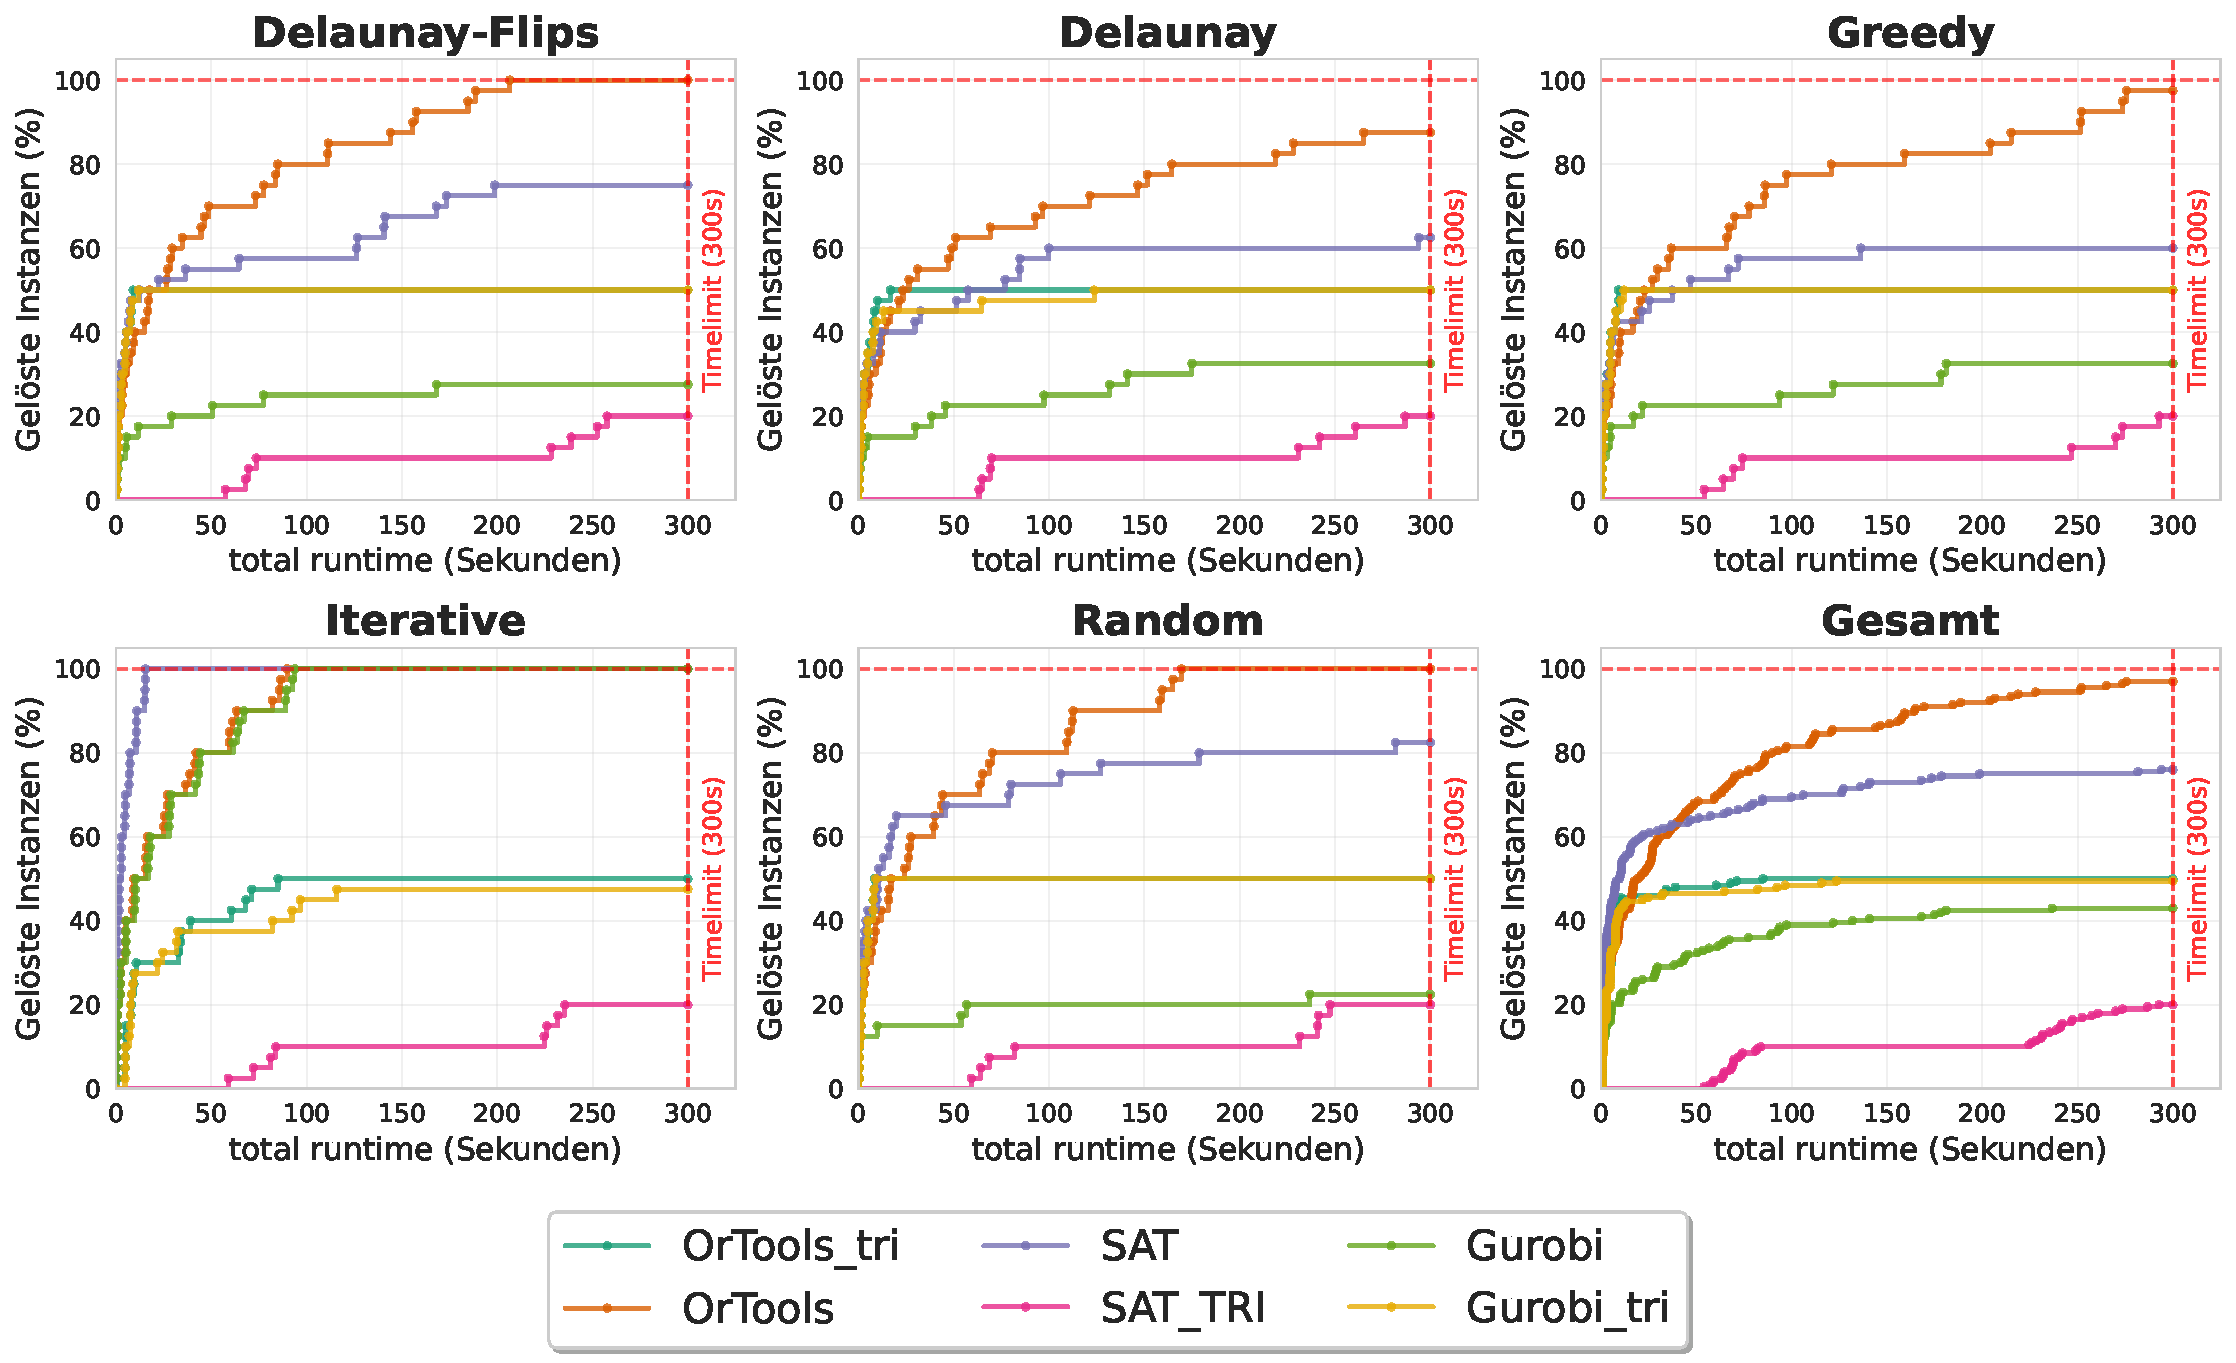
\includegraphics[width=1\linewidth]{figures/eval1/gesamt.pdf}
    \caption{Enter Caption}
\end{figure}

{%
  \catcode`\_=12 % Unterstrich als normales Zeichen
  \catcode`\#=12 % Rautenzeichen als normales Zeichen
    \obeylines
    \input{figures/eval1/gesamt.txt}
}



